\section{Outlook}

% Contributions
\begin{frame}
    \frametitle{Contributions}

    \only<1>{
        \begin{itemize}
            \item Properties of the data set
            \item Penalty ratio metric
            \item Thorough analysis of order methods
            \item Design of order-based LCD
            \item New quantitative and qualitative evaluation approaches
        \end{itemize}
    }

\end{frame}



\begin{frame}
    \frametitle{Outlook}

    % Theoretical questions
    \only<1>{
        Theoretical questions
        \begin{itemize}
            \item Order and positions are inferred from the data
            \item How valid is the exogeneity assumption?
            \item What functional relations between data and context are allowed?
            \item What implicit assumptions are required for the current method?
        \end{itemize}
    }

    % Further testing: simulation, different data
    \only<2>{
        Further testing
        \begin{itemize}
            \item Simulation
            \item Different data sets
        \end{itemize}
    }

    % Method adaptation: gradual and radical
    \only<3>{
        Adaptations to the method
        \begin{itemize}
            \item Gradual
                \begin{itemize}
                    \item More spread-out position estimates
                \end{itemize}
            \item Radical
                \begin{itemize}
                    \item Using continuous data
                    \item Joint estimate of order and position
                    \item Partial order
                    \item More use of known intervention targets
                \end{itemize}
        \end{itemize}
    }

    % Back to statistical and symbolic synergy: symbolic AI is hard
    \only<4>{
        \frametitle{One Step Closer to Human-Level Machine-Intelligence?}

        \begin{center}
            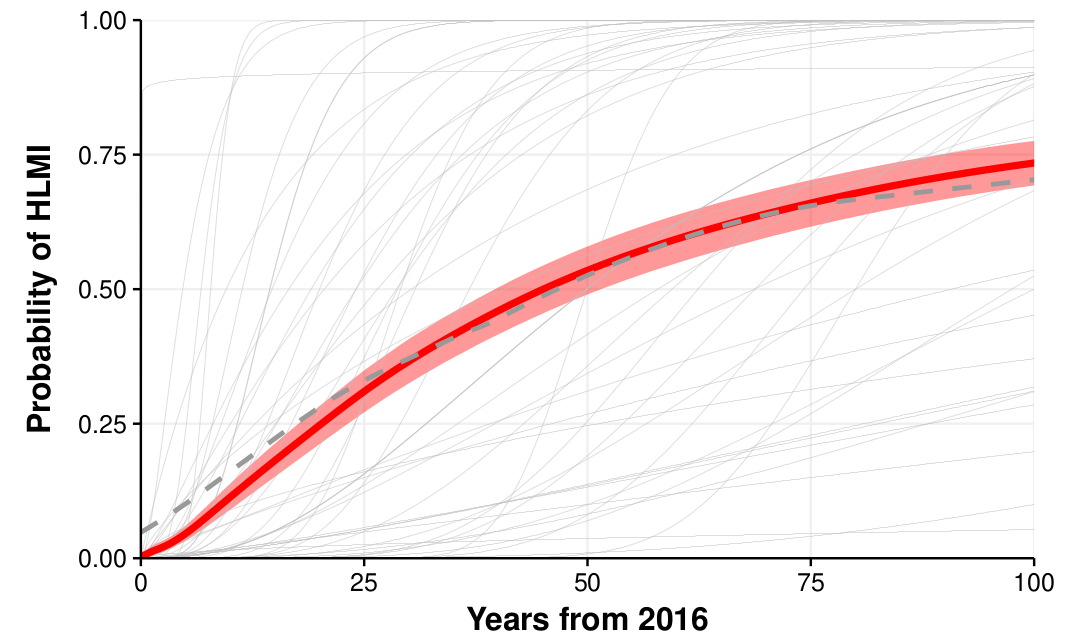
\includegraphics[width=.8\textwidth]{1introduction/hlmi.png}
        \end{center}

    }
    

\end{frame}